\chapter{Wykorzystane narzędzia i technologie}
\label{cha:wykorzystaneNarzedziaITechnologie}
W niniejszym rozdziale zostaną zawarte krótkie opisy narzędzi oraz technologii wykorzystanych w trakcie implementacji algorytmu będącego tematem owej pracy inżynierskiej. Zostanie również przedstawiony język programowania, w którym stworzono projekt, oraz charakteryzujące go zalety przeważające o jego wyborze. 

% %---------------------------------------------------------------------------

\section{Python}
Język programowania Python \cite{PythonWiki} powstał we wczesnych latach dziewięćdziesiątych. Guido van Rossum jest uważany za głównego twórcę tego języka, jednak wkład w jego rozwój miały także inne osoby. 

\begin{figure}[h]
	\centering
	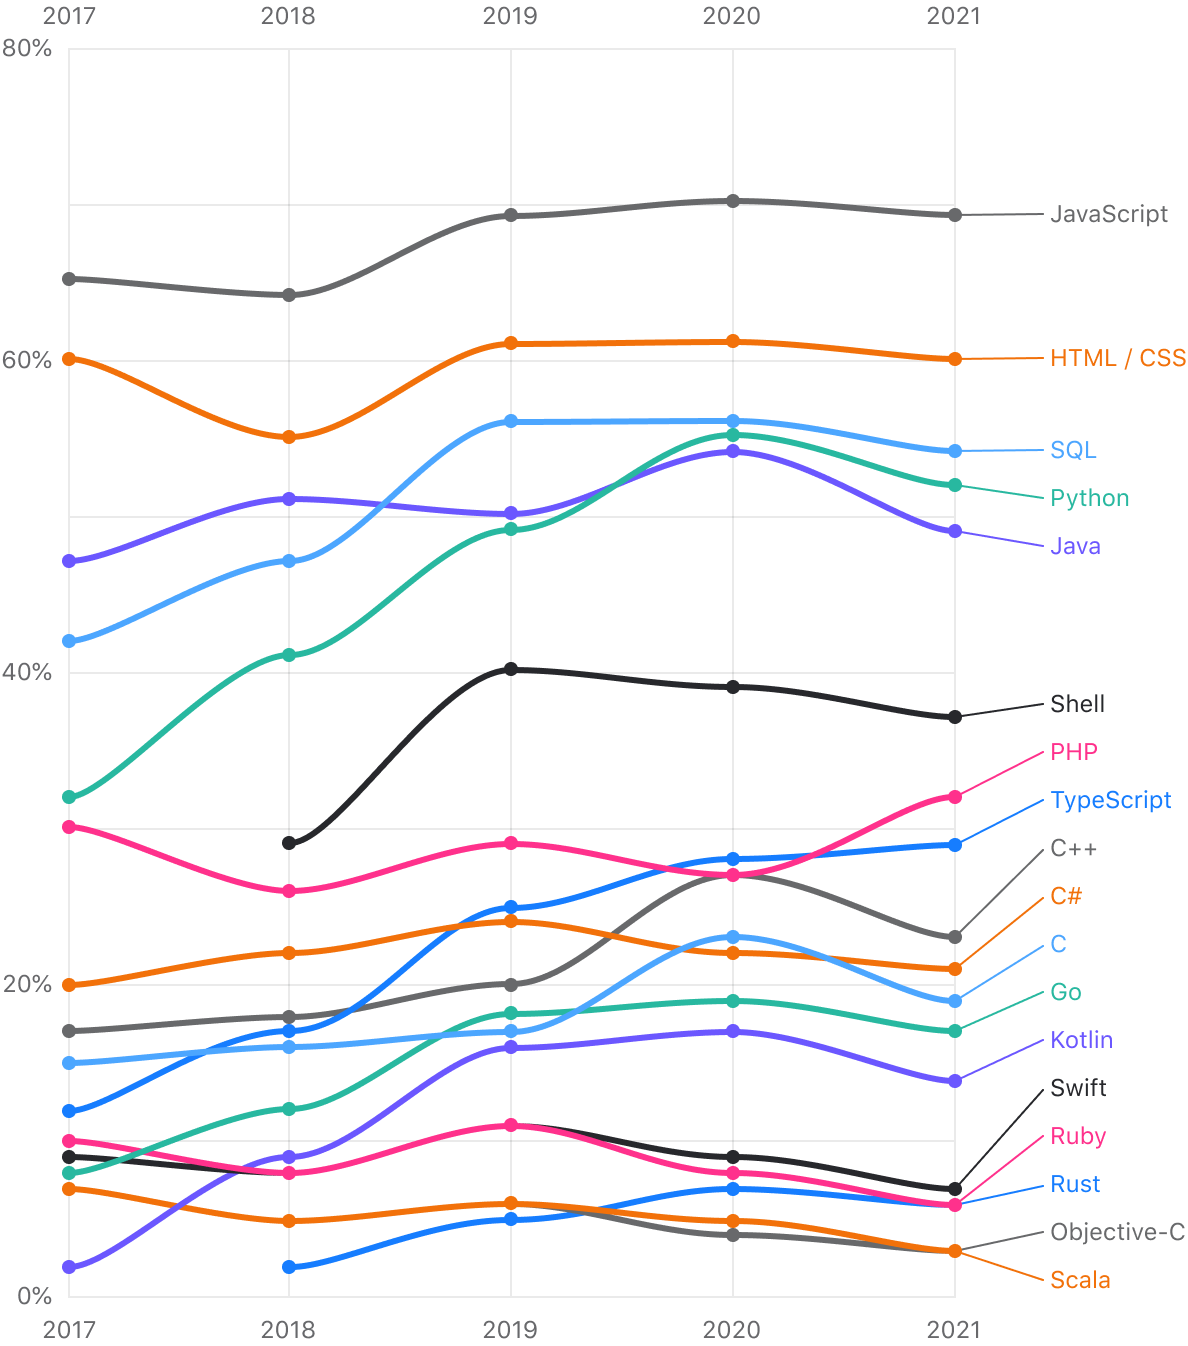
\includegraphics[width=8cm]{zdjęcia/python.png}
	\caption{Popularność języków programowania na przestrzeni lat \cite{pythonLanguages}} 
	\label{fig:programmingLang}
\end{figure}

Popularność narzędzia wzrosła diametralnie w momencie wydania wersji $2.0$ w roku 2000 i rośnie aż do teraz. Aktualnie znajduje się on w czołówce najczęściej wykorzystywanych języków (Rys. \ref{fig:programmingLang}). Jego interpretery dostępne są dla wielu systemów operacyjnych, obsługuje większość używanych w dzisiejszych czasach platform, takich jak Windows, Linux, AIX, iOS i inne.

Projekt, w ramach którego zostaje rozwijany owy język zarządzany jest przez Python Software Foundation, będącą organizacją non-profit. Narzędzie zostało udostępnione jako otwarte oprogramowanie, przez co użytkownicy posiadają możliwość ingerowania w wydawany kod źrodłowy.

Python to język wielopoziomowy, którego przeznaczenie nie jest ściśle określone. Jego możliwości są niezwykle rozległe i uzależnione od stosowanych bibliotek, platform oraz gotowych skryptów, których wybór jest wyjątkowo obszerny. 

Język nie wymusza od użytkownika jednego stylu, w którym tworzone są programy. Istnieje możliwość zastosowania różnych paradygmatów programowania (obiektowe, strukturalne oraz funkcyjne), co zdecydowanie wpływa na rozległość jego zastosowań. Ważną cechą jest także dynamiczna typizacja, którą oferuje. Podczas tworzenia zmiennych nie wymaga się definiowania ich typu. Co więcej Python posiada automatyczne zarządzanie pamięcią, które zwalnia programistę z tego obowiązku. 

\begin{figure}[h]
	\centering
	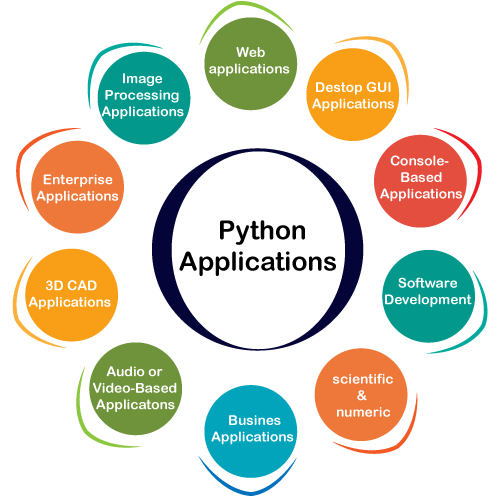
\includegraphics[width=7cm]{zdjęcia/python_usage.png}
	\caption{Dziedziny, w których najczęściej wykorzystuje się język programowania Python \cite{PythonApps}} 
	\label{fig:pythonUsage}
\end{figure}

Główną ideą towarzyszącą twórcy podczas opracowywania składni języka była wysoka czytelność kodu źródłowego, jego przejrzystość i zwięzłość. Okazało się to jednym z głównych czynników, które spowodowały, że stał się tak powszechnie wykorzystywany.

Dzięki swojej uniwersalności Python odnajduje zastosowanie w wielu różnych dziedzinach, które zostały przedstawione na Rys. \ref{fig:pythonUsage}. 

Popularność w środowisku matematycznym zawdzięcza bibliotece SciPy stanowiącą darmową alternatywę do języka Matlab. Biblioteka Tensor Flow wspiera tworzenie sieci neuronowych, wykorzystywane w tworzeniu algorytmów w popularnych aplikacjach \cite{PythonApps}. W przypadku dziedzin operujących na przetwarzaniu obrazów czy też analizowaniu danych Python dostarcza kilka pakietów ułatwiających te operacje.

Ze względu na powyższe fakty, to jest między innymi czytelność, uniwersalność oraz ogromne zasoby pakietów, algorytm będący tematem niniejszej pracy inżynierskiej został opracowany w języku Python. W następnej sekcji zostaną przedstawione biblioteki wykorzystane w~jego implementacji.

% %---------------------------------------------------------------------------

\section{Biblioteki}
Biblioteki programistyczne dostarczają podprogramy, które użytkownik może wykorzystać w swoim kodzie źródłowym bez konieczności implementowania ich od podstaw. Jest to metoda na wielokrotne używanie identycznego kodu.

% %---------------------------------------------------------------------------

\subsection{OpenCV}
Biblioteka OpenCV \cite{opencv} jest narzędziem wydanym jako otwarte oprogramowanie, wspomagające przetwarzanie obrazów oraz uczenie maszynowe. Została napisana w języku C, natomiast posiada interfejsy dla innych języków, takich jak Java, Python bądź Matlab.

Zawiera około 2500 zoptymalizowanych algorytmów implementujących między innymi wykrywanie i rozpoznawanie twarzy, identyfikację i śledzenie ruchu obiektów. Znajdują się w niej także moduły dotyczące modeli 3D, ich tworzenia i przetwarzania.

Poza skomplikowanymi algorytmami OpenCV dostarcza wiele podstawowych operacji, które wykorzystuje się przy modyfikacji obrazów. Zaimplementowane funkcje zdają się wyróżniać wydajnością, co jest bardzo istotne w przypadku działania na dużych zbiorach danych.

% %---------------------------------------------------------------------------

\subsection{imutils}
Pakiet imutils \cite{imutils} to kolejne przydatne narzędzie wykorzystywane w trakcie modyfikacji obrazów. Zawiera szereg funkcji ułatwiających ich przetwarzanie, takich jak obracanie, zmiana rozmiaru, przesunięcie, zastosowanie szkieletyzacji. Zaimplementowano także moduły ułatwiające poprawną prezentację zdjeć podczas ich wyświetlania.

Funkcje zawarte w owym pakiecie pochodzą z biblioteki OpenCV, zostały one odpowiednio połączone i zmodyfikowane, aby można było w prostszy sposób dokonywać podstawowych operacji na zdjęciach. Biblioteka OpenCV zawiera ogromną ilość komponentów, co może być przytłaczające dla osoby rozpoczynającej swoją przygodę z przetwarzaniem obrazów.

Ideą, dla której powstał ten pakiet była chęć zebrania podstawowych modułów i odpowiednie ich dostosowanie w celu ograniczenia zbędnych operacji, które należy zastosować korzystając z biblioteki OpenCV.

% %---------------------------------------------------------------------------

\subsection{dlib}
Dlib to biblioteka udostępniona na zasadach otwartej licencji, napisana w języku C++ \cite{dlib}. Dostarcza ona algorytmy oparte na uczeniu maszynowym oraz narzędzia do tworzenia oprogramowania we wspomnianym wyżej języku. 

Funkcje, z których można korzystać, implementują algorytmy umożliwiające wytrenowanie klasyfikatorów SVM oraz SVR. Dodatkowo istnieje możliwość wytrenowania własnego modelu wykrywającego twarz lub jej punkty charakterystyczne.

Zastosowania tej biblioteki obejmują takie dziedziny jak przemysł, robotyka oraz wszelkie obszary wymagające skorzystania z programów o dobrej wydajności obliczeniowej.

% %---------------------------------------------------------------------------

\subsection{scikit-image}
Biblioteka scikit-image \cite{skimage}, podobnie jak opisane powyżej pakiety, zawiera szereg implementacji algorytmów powiązanych z przetwarzaniem obrazów. Została ona udostępniona jako otwarte oprogramowanie tworzone przez kilkadziesiąt osób. 

Obejmuje takie algorytmy jak transformacje, segmentacje obrazów, ich morfologię oraz manipulację przestrzenią kolorów. Pakiet korzysta z tablic biblioteki NumPy, wykorzystanych do przechowywania obrazów.

% %---------------------------------------------------------------------------

\section{Flask}
Flask \cite{flask} to minimalistyczny szkielet wspierający tworzenie aplikacji webowych (ang. microframework). Zawiera wiele przydatnych bibliotek oraz modułów umożliwiających ich proste implementowanie.

W odróżnieniu od pełnowymiarowej platformy programistycznej (ang. framework) nie posiada warstwy abstrakcji bazy danych, części walidacyjnej formularzy czy też innych elementów, które wymagałaby zapewnienia szczególnych bibliotek. Natomiast obsługuje rozszerzenia, ktore umożliwiają dodanie owych funkcji do aplikacji.

Flask dostarcza programiście wiele przydatnych modułów, dzięki którym nie musi się on zajmować obsługą wątków i protokołów. Oparty jest na zestawie kilku narzędzi, na które składają się:
\begin{itemize}
\item \textit{Werkzeug} - biblioteka udostępniająca zestaw narzędzi WSGI (ang. Web Server Gateway Interface) rozumianych jako interfejs bramy serwera WWW. Implementuje on przetwarzanie żądań między serwerem a aplikacją.
\item \textit{jinja2} - biblioteka programistyczna umożliwiająca osadzanie danych na stronie w odpowiednich szablonach prezentacyjnych, której rezultat jest widoczny w przeglądarce.
\item \textit{MarkupSafe} - biblioteka rozszerzająca typ tekstowy, zapewniająca bezpieczne używanie znaków w HTML oraz XML. Zabezpieczna przed atakami poprzez wprowadzanie niezaufanych danych.
\item \textit{ItsDangerous} - pakiet odpowiadający za poprawną serializację danych. Służy do przechowywania sesji za pomocą plików cookies.
\end{itemize}

Głównymi zaletami opisywanego szkieletu jest jego prostota i brak ograniczeń związanych ze ściśle ustalonymi regułami, którymi należy się kierować budując program. Jest niezwykle elastyczny, nadaje się do tworzenia małych, wewnętrznych aplikacji, ale jednocześnie daje możliwość rozbudowania ich do pełnowymiarowej struktury. 

W związku z wymienionymi zaletami, Flask zdaje się być idealnym narzędziem do stworzenia prostej aplikacji mającej na celu walidację algorytmu tworzonego w owym projekcie.

% %---------------------------------------------------------------------------

\section{Pycharm}
Pycharm \cite{pycharm} jest zintegrowanym środowiskiem wspierającym dla języka programowania Python. Oprogramowanie jest dostępne na wielu platformach systemowych takich jak Windows, Linux i macOS. Oferuje inteligentny edytor kodu źródłowego z możliwością formatowania i autouzupełniania, który posiada funkcję weryfikacji błędów oraz ich kontrolowanie.

Zapewnia refaktoryzację języka, przez co utrzymana jest wysoka jakość systemowa. Elementy są wpasowywane w dane wzorce, dopasowywane do obowiązujących standardów.

Ważną kwestią jest udostępniane wsparcie dla różnych bibliotek i narzędzi. Pycharm wspiera tworzenie stron internetowych z wykorzystaniem biblioteki Django, czy też Flaska i Pyramid. Wspomaga tworzenie plików w językach powiązanych z technologią webową (HTML, CSS, JavaScript).

Ułatwia pracę z projektem dostarczając prosty interfejs konfiguracyjny. W przypadku tworzenia aplikacji webowej opartej na platformie Flask w nieskomplikowany sposób można wprowadzić wszystkie istotne ustawienia.






